\documentclass[11pt]{article}
\usepackage[T1]{fontenc}
\usepackage[utf8]{inputenc}
\usepackage{lmodern,amsmath,amssymb,graphicx,geometry,microtype,setspace,booktabs,caption}
\usepackage[hidelinks]{hyperref}
\geometry{letterpaper,margin=1in}
\setlength{\parindent}{0pt}
\setlength{\parskip}{0.55em}
\setlength{\emergencystretch}{2em}
\captionsetup{labelfont=bf,font=small}
\renewcommand{\refname}{References}

\pagestyle{empty}
\renewcommand{\thefigure}{S\arabic{figure}}
\setcounter{figure}{4}

\begin{document}
\begin{figure}[!ht]\centering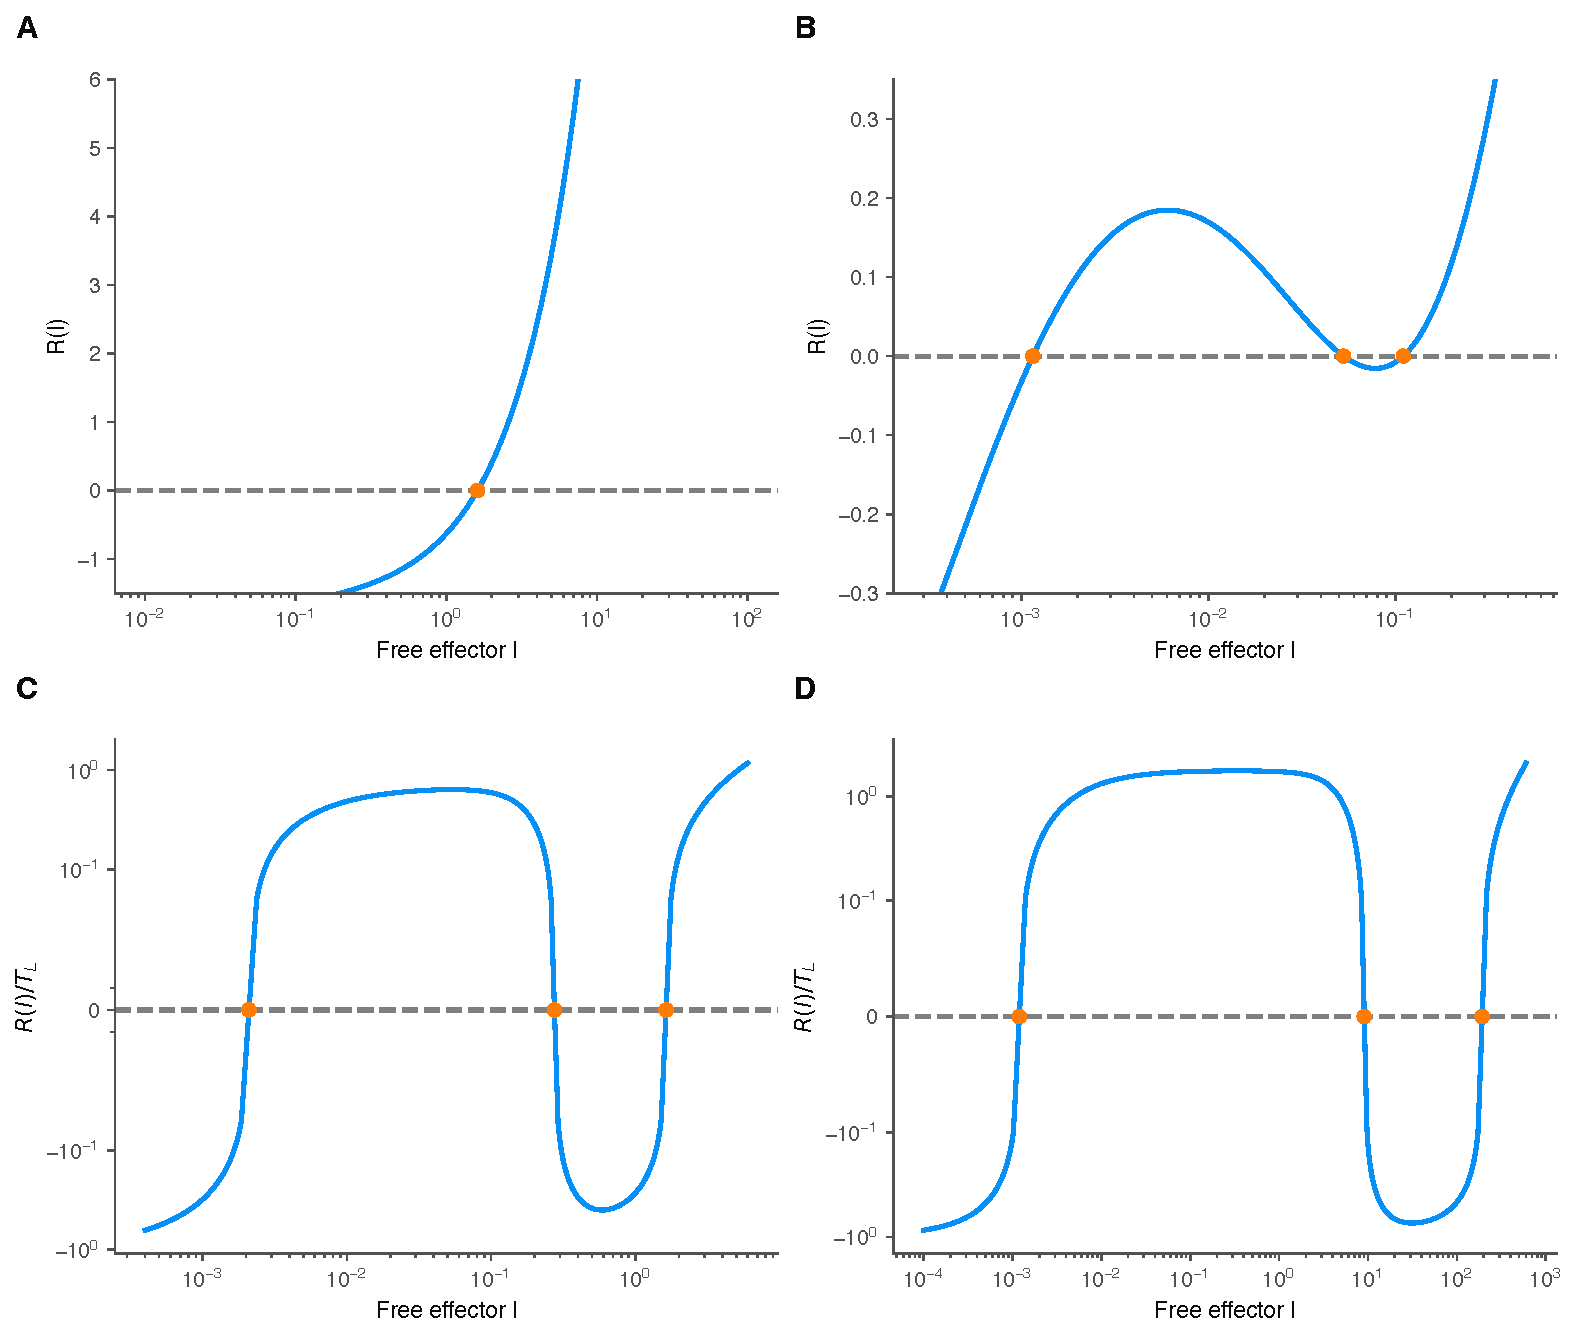
\includegraphics[width=\textwidth,height=0.65\textheight,keepaspectratio]{figure_inputs/FigS5_uniqueness.pdf}\begin{singlespace}\caption{Uniqueness conditions and verified multistationarity. (A) Corrected independent-site kinetic example satisfying both conditions. (B) Original four-site example with catalytic-ratio spread 2.89: three positive states, but both conditions are violated. (C) Constant catalytic ratios with condition (ii) violated. (D) An exact binomial ladder satisfying condition (ii) globally, with condition (i) violated and three physical states. Panels C and D use residual divided by total effector with symmetric logarithmic vertical axes. Markers are refined roots, not neighboring grid points. S11 and S1 Data specify all parameters, positivity checks, and the exact root count for D. Stability is not encoded by the marker style.}\end{singlespace}\end{figure}
\end{document}
